\documentclass[11pt,a4paper]{article}
\usepackage[utf8]{inputenc}
\usepackage[T1]{fontenc}
\usepackage{amsmath}
\usepackage[usenames,dvipsnames,svgnames,table]{xcolor}
\usepackage[normalem]{ulem}
\usepackage[left=1.00cm, right=1.00cm, top=0.40cm, bottom=0.2cm]{geometry}
\PassOptionsToPackage{defaults=hu-min}{magyar.ldf}
\usepackage[magyar]{babel}
\usepackage{framed, fancyhdr, wasysym, graphicx, multirow, hyperref}

\begin{document}
\renewcommand{\labelitemi}{\textbullet}
\def\br{\\[0.1cm]}
\thispagestyle{empty}
\begin{center}
	\colorbox{lightgray}{{\large JPSMA3} \hspace{3cm} {\large Webes alkalmazások fejlesztése 2. beadandó} \hspace{5cm} \thepage}
\end{center}
\begin{framed}
	\begin{flushleft}
		{\large \textbf{Bauer Bence}}
		\hspace{3cm}{\large \textbf{2.Beadandó/9.Feladat}}
		\hspace{5.4cm}{\large 2019.05.12.}\br
		{\large JPSMA3}\br
		{\large \href{mailto:bauerbence5@gmail.com}{bauerbence5@gmail.com}}
	\end{flushleft}
\end{framed}
\section{Feladat}
Asztali grafikus felület, melyet az alkalmazottak használnak a
mozipénztárakban az előadások meghirdetésére, illetve jegyek kiadására.
\begin{itemize}
\item Az alkalmazott bejelentkezhet (felhasználónév és jelszó megadásával) a
programba, illetve kijelentkezhet.
\item Új film felvitelekor ki kell tölteni a film adatait (cím, rendező,
hossz, szinopszis), valamint feltölthetünk egy képet plakátként.
\item Új előadás meghirdetéséhez a felhasználónak ki kell választania a termet,
valamint a filmet, és az időpont megadásával hirdetheti meg az előadást. A
meghirdetéskor ügyelni kell arra, hogy az előadás ne ütközzön más
előadásokkal az adott teremben (figyelembe véve a kezdés időpontját, illetve
a film hosszát), illetve két előadás között legalább 15 percnek kell eltelnie a
takarítás végett.
\item A jegyvásárláshoz ki kell választani a filmet és az előadást. Ezt követően
listázódnak a helyek (sor, oszlop, státusz). A szabad, illetve foglalt helyek
eladhatóak, illetve a foglalt helyeket kiválasztva meg lehet tekinteni a foglaló
adatait (név, telefonszám).
\end{itemize}
Az adatbázis az alábbi adatokat tárolja:
\begin{itemize}
\item filmek (cím, rendező, szinopszis, hossz, plakát, bevitel dátuma)
\item termek (név, sorok száma, oszlopok száma)
\item előadások (film, kezdő időpont, terem)
\item helyek (előadás, terem, sor, oszlop, státusz
<szabad, foglalt, eladott>, foglaló, neve, foglaló telefonszáma)
\item alkalmazottak (teljes név, felhasználónév, jelszó)
\end{itemize}

\section{Elemzés}
\begin{itemize}
\item Az alkalmazás perzisztencia részét egy külső C\# könyvtárként kezeljük.
A weblap részt MVC segítségével hozzuk létre. A grafikus felületet WPF-el MVVM
architektúrában megvalósítva.
\item Több ablakra is szükségünk van:
\begin{itemize}
	\item Bejelentkező felület
	\item Egy menüablak, ahol kiválaszthatjuk melyik funkciót szeretnénk használni
	\item Valamint egy ablak minden funkciónak (Új film felvétele, új előadás felvétele,
	jegyeladás rögzítése)
\end{itemize}
\item Az alkalmazáshoz szükséges egy adatbázis is. A feladatban leírt adatbázis jól
megfogalmazható SQL adatbázisként.
\end{itemize}

\newpage
\begin{center}
\colorbox{lightgray}{{\large JPSMA3} \hspace{3cm} {\large Webes alkalmazások fejlesztése 2. beadandó} \hspace{5cm} \thepage}
\end{center}
\begin{figure}[h]
\centering
\includegraphics[width=10cm]{umls/usecase.png}
\caption{Felhasználói eset diagram}
\end{figure}

\section{Tervezés}
\begin{itemize}
\item Programszerkezet
\begin{itemize}
	\item A programot MVVM architektúrával valósítjuk meg.
	\item A feladathoz a programot két projektre osztjuk. Egy a Cinema.Persistence, mely
	az adatbázis létrehozását és a használt típusait kezeli.
	\item A másik projekt a Cinema.WPF felelős az app futtatásáért, illetve a funkcióiért.
	Itt találhatóak a View-ViewModel párok, melyekkel megvalósítjuk a különböző oldalakat.
\end{itemize}
\begin{figure}[h]
\centering
\includegraphics[width=10cm]{umls/szerkezet.png}
\caption{Az app és a perzisztencia szerkezete}
\end{figure}

\newpage
\begin{center}
\colorbox{lightgray}{{\large JPSMA3} \hspace{3cm} {\large Webes alkalmazások fejlesztése 2. beadandó} \hspace{5cm} \thepage}
\end{center}

\item Perzisztencia
\begin{figure}[h]
	\centering
	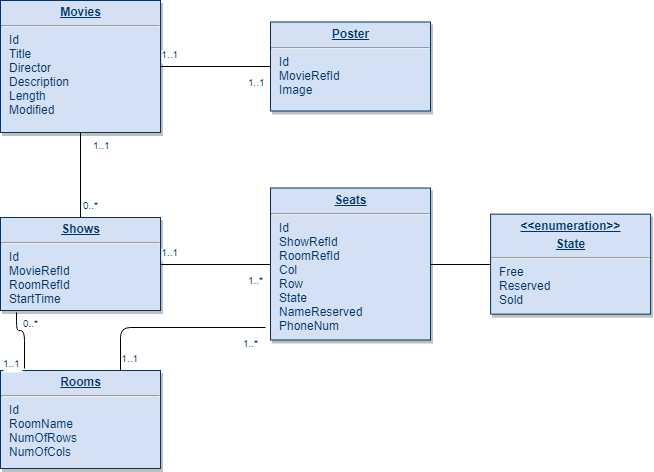
\includegraphics[width=12cm]{umls/Entity.png}
	\caption{Adatbázis felépítése}
\end{figure}

\item WPF alkalmazás
\begin{itemize}
	\item WPF alkalmazás MVVM architektúrában megvalósítva
	\item Services, mely a szerver oldali hívásokat végzi
	\item Szükséges nézetek:
	\begin{itemize}
		\item Login - Bejelentkezés
		\item Menu - Főmenü
		\item NewMovie - Új film felvétele
		\item NewShow - Új előadás felvétele
		\item Reservation - jegyeladás
	\end{itemize}
	\item Minden nézethez tartozik egy ViewModel is
\end{itemize}

\item WebAPI
\begin{itemize}
\item api/Account/\{username\}/\{password\}:\\[0.1cm]
HttpGet - Bejelentkezés
\item api/Account/Logout:\\[0.1cm]
HttpGet - Kijelentkezés
\item api/Movie\\[0.1cm]
HttpGet - Filmek lekérdezése\\[0.1cm]
HttpPost - Új film felvétele
\item api/Reservation/SeatList/\{id\}\\[0.1cm]
HttpGet - Az előadáshoz tartozó ülőhelyek lekérdezése
\item api/Reservation\\[0.1cm]
HttpPost - Jegyeladás rögzítése
\item api/Show/ShowList\\[0.1cm]
HttpGet - Elérhető előadások lekérdezése
\item api/Show/RoomList\\[0.1cm]
HttpGet - Mozitermek lekérdezése
\item api/Show\\[0.1cm]
HttpPost - Új előadás felvétele
\end{itemize}
\end{itemize}

\section{Tesztelés}
A webszolgáltatás tesztelése Unit teszteken keresztül történt, egy memóriában létrehozott
adatbázis használatával.
\begin{itemize}
	\item\textit{GetMoviesTest:} Filmek lekérdezésének tesztelése.
	\item\textit{GetShowsTest:} Előadások lekérdezésének tesztelése.
	\item\textit{GetRoomsTest:} Mozitermek lekérdezésének tesztelése.
	\item\textit{AddNewMovieTest:} Új film hozzáadásának tesztelése.
	\item\textit{AddNewShowTest:} Új előadás hozzáadásának tesztelése.
	\item\textit{ReservationTest:} Jegyeladás rögzítésének tesztelése.
\end{itemize}

\end{document}